\documentclass[../main.tex]{subfiles}
\begin{document}
\clearpage
\refstepcounter{section}
\section*{Приложение \Alph{section}.  Свидетельства о государственной регистрации программ для ЭВМ}% Заголовок с "Приложение A"
\label{app:B}% Метка с буквой (например, app:A)
\addcontentsline{toc}{section}{Приложение \Alph{section}. Свидетельства о государственной регистрации программ для ЭВМ}% Добавляем в оглавление
\renewcommand{\theequation}{\Alph{section}.\arabic{equation}}% Формат A.1 для формул
\setcounter{equation}{0}
 	\begin{figure}[h]
 		\centering
 			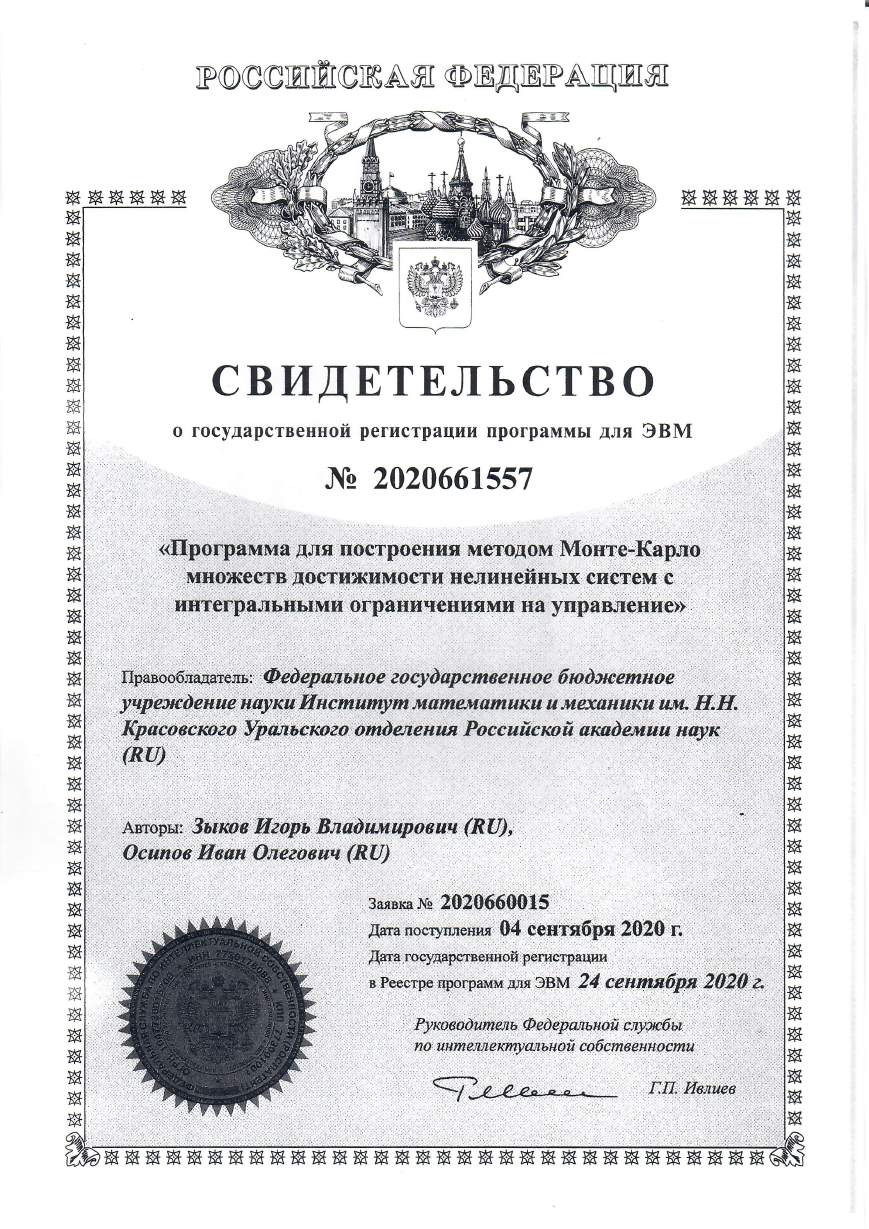
\includegraphics[width=0.8\textwidth]{images/ZykovOsipovPatent.jpg}
 	\end{figure}
\end{document}